% UG project example file, February 2024
%
%   Added the "online" option for equal margins, February 2024 [Hiroshi Shimodaira, Iain Murray]
%   A minor change in citation, September 2023 [Hiroshi Shimodaira]
%
% Do not change the first two lines of code, except you may delete "logo," if causing problems.
% Understand any problems and seek approval before assuming it's ok to remove ugcheck.
\documentclass[logo,bsc,singlespacing,parskip,online]{infthesis}
\usepackage{ugcheck}


% Include any packages you need below, but don't include any that change the page
% layout or style of the dissertation. By including the ugcheck package above,
% you should catch most accidental changes of page layout though.

\usepackage[nopatch=footnote]{microtype} % recommended, but you can remove if it causes problems
\usepackage[round]{natbib} % recommended for citations
\usepackage{graphicx}
\usepackage{xcolor}

\begin{document}
\begin{preliminary}

\title{This is the Project Title}

\author{Jamie Day}

% CHOOSE YOUR DEGREE a):
% please leave just one of the following un-commented
%\course{Artificial Intelligence}
%\course{Artificial Intelligence and Computer Science}
%\course{Artificial Intelligence and Mathematics}
%\course{Artificial Intelligence and Software Engineering}
%\course{Cognitive Science}
%\course{Computer Science}
%\course{Computer Science and Management Science}
%\course{Computer Science and Mathematics}
%\course{Computer Science and Physics}
%\course{Software Engineering}
\course{Master of Informatics} % MInf students

% CHOOSE YOUR DEGREE b):
% please leave just one of the following un-commented
\project{MInf Project (Part 1) Report}  % 4th year MInf students
%\project{MInf Project (Part 2) Report}  % 5th year MInf students
%\project{4th Year Project Report}        % all other UG4 students


\date{\today}

\abstract{
This skeleton demonstrates how to use the \texttt{infthesis} style for
undergraduate dissertations in the School of Informatics. It also emphasises the
page limit, and that you must not deviate from the required style.
The file \texttt{skeleton.tex} generates this document and should be used as a
starting point for your thesis. Replace this abstract text with a concise
summary of your report.
}

\maketitle

\newenvironment{ethics}
   {\begin{frontenv}{Research Ethics Approval}{\LARGE}}
   {\end{frontenv}\newpage}

\begin{ethics}

This project was planned in accordance with the Informatics Research
Ethics policy. It did not involve any aspects that required approval
from the Informatics Research Ethics committee.

\standarddeclaration
\end{ethics}


%\begin{acknowledgements}
%I would like to thank Saj's Shawarma and Grill, for always having my back through these hard times.
%\end{acknowledgements}


\tableofcontents
\end{preliminary}


\chapter{Introduction}

The preliminary material of your report should contain:
\begin{itemize}
\item
The title page.
\item
An abstract page.
\item
Declaration of ethics and own work.
\item
Optionally an acknowledgements page.
\item
The table of contents.
\end{itemize}

As in this example \texttt{skeleton.tex}, the above material should be
included between:
\begin{verbatim}
\begin{preliminary}
    ...
\end{preliminary}
\end{verbatim}
This style file uses roman numeral page numbers for the preliminary material.

The main content of the dissertation, starting with the first chapter,
starts with page~1. \emph{\textbf{The main content must not go beyond page~40.}}

The report then contains a bibliography and any appendices, which may go beyond
page~40. The appendices are only for any supporting material that's important to
go on record. However, you cannot assume markers of dissertations will read them.

You may not change the dissertation format (e.g., reduce the font size, change
the margins, or reduce the line spacing from the default single spacing). Be
careful if you copy-paste packages into your document preamble from elsewhere.
Some \LaTeX{} packages, such as \texttt{fullpage} or \texttt{savetrees}, change
the margins of your document. Do not include them!

Over-length or incorrectly-formatted dissertations will not be accepted and you
would have to modify your dissertation and resubmit. You cannot assume we will
check your submission before the final deadline and if it requires resubmission
after the deadline to conform to the page and style requirements you will be
subject to the usual late penalties based on your final submission time.

\section{Using Sections}

Divide your chapters into sub-parts as appropriate.

\section{Citations}

When citing work using author names, your sentences should still read
as correct English if any parts in parenthesis are removed.
Use {\tt {\textbackslash}citet} when citing the name as text that's part of your sentence: 
%\begin{quote}
%  We follow the method of \citet{P1}.
%\end{quote}
%and use {\tt {\textbackslash}citep} for a parenthetical citation:
%\begin{quote}
%  It's possible to learn first-order Horn sequences from entailment \citep{P2}.
%\end{quote}

You may use any consistent reference style that you prefer, including ``[1]'' numerical citations. 








\chapter{Context}

\section{What are effect handlers?}
Effect handlers and the associated effects are a type of control flow pattern that have many applications, including for backtracking, cooperative multi-threading and more.\cite{effect_handlers_tutorial} A programmer will define specific \textit{effects}, and instantiate specific \textit{effect handlers} that will handle all effects of a predetermined type that are called within its scope. For example: 

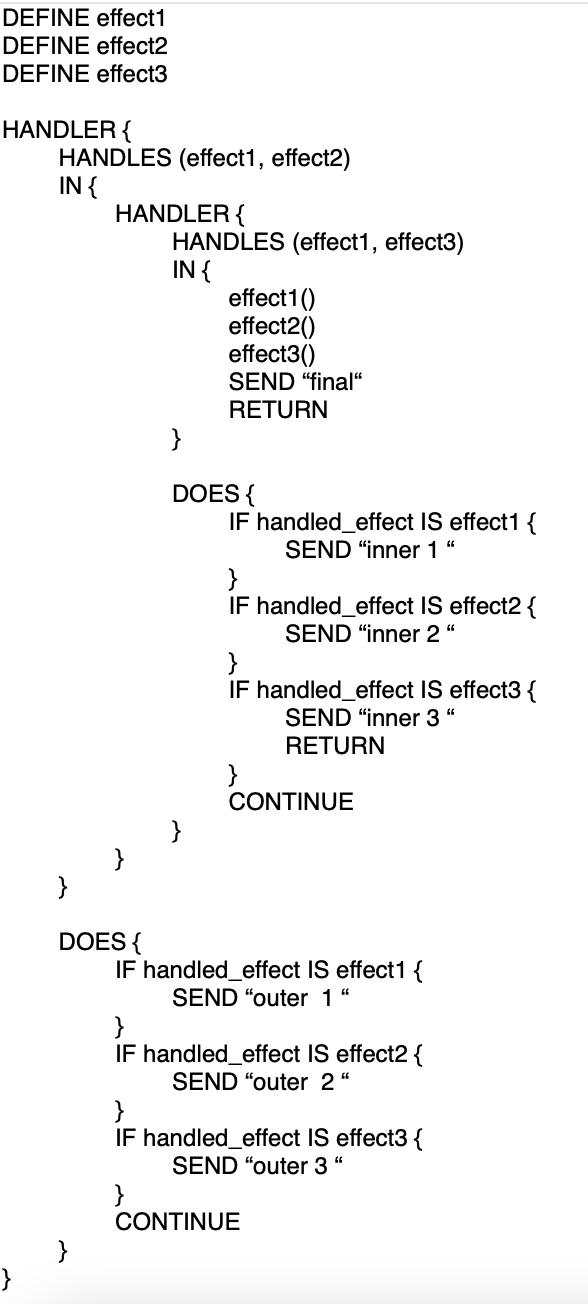
\includegraphics[scale=0.4]{pseudocode_handler.png}

Here the output would be "inner 1 outer 2 inner 3 ". Note that this does not include the output "final" - the continuation does not have to be resumed after the error is handled. Note also that we can consider the second inner IF (that prints "inner 2 ") and the third outer IF to be dead code, since they don't handle this effect.

The key part to notice is what happens with effect 2 - the effect call "bubbles up" the stack of effect handlers until it finds a handler that can handle it. This is a key concept when it comes to effect handlers.

Note that since the inner handler does not handle the \textbf{[name]} effect, the effect call continues bubbling up the call stack until it finds the first handler that does handle it. This compositionality is essential to effect handlers usefulness %[rewrite this sentence].







\section{What is libseff?}

Although much of the current usage of effect handlers is found in functional languages, there exist libraries that implement effect handling in almost every major language in which it is possible, including C. However, these libraries, such as \textbf{libmpeff}, are mostly designed specifically for compiler implementation, and as such offer features and make implementation decisions that do not necessarily make sense for the generic use case.\cite{libmprompt} \textbf{libseff}, on the other hand, is an implementation of effect handlers for C that is designed to be used directly by programmers.\cite{libseff_paper}

Currently defining an effect looks like this: %[image]

and calling it looks like this: %[image]

You may note that when defining the effect it is necessary to pass an integer id that defines the effect. This is a necessary detail of the current implementation of \textbf{libseff}: which effects a specific handler handles are stored as a single 64-bit integer, where each bit represents whether a handler represents that index of effect. This means that the number of IDs is limited to 64, meaning there can be at most 64 different  effects defined in a \textbf{libseff} program. This is the problem that this study will aim to solve.

This was implemented to increase speed at runtime, since this is a priority of the original \textbf{libseff} implementation. %[cite here]  

A further problem with this approach is that IDs must be independent even between libraries, which is unintuitive and generally makes including libraries that use libseff unnecessarily complicated, since it is necessary to ensure that the ids of effects do not collide, and the maximum limit of 64 effects may start to become relevant in this case.

This may cause unpredictable errors, since [cite 2.1 of the paper] errors are only caused when handlers with the same id are interlaced and then an effect is called that is meant to be handled by the handler higher in the heirarchy, but is handled by the lower one because the ids match. This doesn't cause an exception but fails silently and unpredictably which is a recipe for chaos. %[change this]

\chapter{Changes Made}

\section{ID assignment}

As stated above, in libseff effect IDs must be assigned manually by the programmer, which causes many issues. A goal of this project was to have some method for assigning IDs automatically, with the following requirements:

 - IDs must be unique: no two effects can have the same ID
 - The number of IDs able to be defined must not be bound in any meaningful way
 - Given the above constraints, checking whether a handler handles a given effect should be as fast as possible

First we turn our attention to ID generation. As widely noted [CITE HERE], Universally Unique Identifiers (UUIDs) can be generated through the use of a so-called "magic pointer" [CITE PLS], or a pointer to a fixed location in memory. Since pointers in C are guaranteed by the standard to only compare equal if they point to the same location [CITE], (as perhaps you would expect), if a new memory address is assigned for each new effect, IDs generated this way are guaranteed to be unique. In this particular case, user-defined effect IDs are actually a pointer to the address that stores where the default generator for that effect is (it's a double pointer), because this is useful later.

[INSERT CODE IMAGE HERE]

One issue with this is that effect IDs are no longer fixed at compile time, which causes a few innefficiencies - for example, these effects can no longer be used in C's \textcolor{teal}{case} statements. Indeed, this cannot be avoided with any implementation that guarantees uniqueness without requiring knowledge of IDs chosen by included libraries, since dynamic libraries are only available at link time.

\section{Effect set representation}

Previously, effect sets were represented as a 64-bit integer, with each bit being 1 implying the handling of the effect with that index as an ID, and similarly 0 means its not handled, as shown below: [INCLUDE IMAGE OF 0s with like 2 ones and some arrows to them that say "this handles effect 3 and effect 12"]

The current solution works more like a string - the effect set is a 0-terminated list of word-length integers, each corresponding to an effect. While this does add another layer of pointer indirection, which had [INSERT EFFECT BELOW] as shown below, it also allows the handling of any number of effects per handler, and importantly also implies that the total number of valid effect IDs is not limited to 64, as the previous implementation implied.

This is a valid representation because 0, the value of the null pointer, is guaranteed to never be allocated by C. Another special ID was also required - a signifier that this handler handles all effects. Although the address 0x1 is not guaranteed to be unallocated by the C standard, virtually every modern implementation of the C compiler allocates the first [X] bytes from 0 as an inacessible page, and it is thouroughly unlikely to be allocated to an effect halfway through a program.

0x1 is therefore used to signify two different things - when used as an effect ID and passed to libseff, the handler acquirer will understand that every handler handles this effect. When used in an effect set, libseff will understand the handler that handles this effect handles every effect - something that was trivial to write under the old system, bur requires special consideration now - we certainly cannot include every possible pointer in a list!

\section{Syntax changes}

These changes required changes to the syntax of the libseff library. Users now no longer have to (and can't) specify the ID of effects they define. More subtly, a common pattern seen even in the libseff code written to test and benchmark the library was for a handler to switch on the ID of an effect after being called - something no longer possible with effect IDs that aren't defined at compile time. These cases were rewritten as macros that inline to simply being if statements instead, which is less efficient but for small switches they were largely being compiled as ifs anyway. [SOURCE SOURCE SOURCE]

This syntax is slightly more unwieldy but ultimately the provided macros are simply syntactic sugar for unpacking the payload and do not need to be used for users to apply the full range of libseff.

\chapter{Evaluation}

bangers one and all. I have never done anything wrong and I never shall.

\chapter{Conclusion}

\section{Final Reminder}

The body of your dissertation, before the references and any appendices,
\emph{must} finish by page~40. The introduction, after preliminary material,
should have started on page~1.

You may not change the dissertation format (e.g., reduce the font size, change
the margins, or reduce the line spacing from the default single spacing). Be
careful if you copy-paste packages into your document preamble from elsewhere.
Some \LaTeX{} packages, such as \texttt{fullpage} or \texttt{savetrees}, change
the margins of your document. Do not include them!

Over-length or incorrectly-formatted dissertations will not be accepted and you
would have to modify your dissertation and resubmit. You cannot assume we will
check your submission before the final deadline and if it requires resubmission
after the deadline to conform to the page and style requirements you will be
subject to the usual late penalties based on your final submission time.

% \bibliographystyle{plain}
\bibliographystyle{plainnat}
\bibliography{refs}


% You may delete everything from \appendix up to \end{document} if you don't need it.
\appendix

\chapter{First appendix}

\section{First section}

Any appendices, including any required ethics information, should be included
after the references.

Markers do not have to consider appendices. Make sure that your contributions
are made clear in the main body of the dissertation (within the page limit).


\end{document}
